\capitulo{5}{Aspectos relevantes del desarrollo del proyecto}
En este apartado se va a comentar el desarrollo que ha tenido el proyecto. Se expondrán todas las líneas de investigación seguidas así como las opciones y las decisiones que se tomaron para resolver estos problemas.

\section{Inicio del proyecto}
Este proyecto parte del trabajos de fin de máster de José Miguel Ramírez Sanz y José Luis Garrido Labrador, tutores de este trabajo, en los que se obtenía un esqueleto por cada \textit{fotograma} de un vídeo de ejercicios y el trabajo de fin de grado de Lucía Nuñéz Calvo en el que se detectaba el inicio y el fin de un ejercicio para poder recortar los vídeos. El conjunto de proyectos, realizados en colaboración con el Hospital Universitario, tienen como objetivo poder mejorar la calidad de vida de los pacientes que padecen enfermedad de \textit{Parkinson} mediante la implementación de un sistema que les permita realizar ejercicios cómodamente desde su hogar y si es posible sin la necesidad de la presencia continua de un terapeuta, haciendo así estas sesiones más frecuentes.

Inicialmente se contemplaron dos temas para el trabajo, la mejora en el sistema de detección de poses y la obtención de una puntuación de los ejercicios realizado por los pacientes comparándolos con el vídeo de un terapeuta, se optó por esta ultima, ya que sin una puntuación que permita saber a los pacientes como de bien han realizado el ejercicio es necesario para que el sistema de telerehabilitación sea viable.

En las primeras semanas se investigó sobre \textit{Detectron} 2, la forma en la que este extraía las poses de los vídeos. Más adelante descubrimos que este proceso no era perfecto, ya que en muchos casos o faltaban posiciones o había demasiado errores en la extracción de estos como que los esqueletos hicieran movimientos imposibles. También se aprendió a utilizar \textit{Docker} ya que es una herramienta con la que no tenía experiencia.

\section{Investigación de métodos para poder puntuar el ejercicio}
En todo proyeto de investigación, el primer paso es realizar un estado del arte para saber que técnicas aplicar y cómo hacerlo. En el caso de este trabajo era vital el poder establecer que era importante a la hora de obtener una puntuación. Inicialmente se investigó cómo conseguían este objetivo juegos de baile como pueden ser \textit{Just Dance} o \textit{Dance Central}.

En la primera investigación no se encontró información oficial por parte de los creadores de dichos juegos excepto un artículo de \textit{Ubisoft} que mencionaba que en juegos anteriores a \textit{Just Dance 2023} bastaba con agitar el mando para conseguir la máxima puntuación \cite{justdance}, por lo que una posible solución que se contemplo al principio fue detectar cambios en la posición para puntuarlo, pero se descarto rápidamente ya que esto no aseguraba que el usuario hubiera realizado correctamente el ejercicio.

Continuando con la investigación se encontró otra posible forma de obtener una puntuación que era mediante el uso de la distancia coseno para comparar los vectores formados por los puntos del esqueleto. Pero esto presentaba otro problema, que se vio al principio del proyecto, la enfermedad de \textit{Parkinson} provoca problemas de movilidad, por lo que, es más probable que la ejecución de los ejercicios sea más rápida en el caso de un fisioterapeuta que en el caso de un paciente. En la figura \ref{fig:longitud} se puede observar esta diferencia, la secuencia del profesional es mucho más corta que la del paciente, lo que complica bastante la comparación.

\begin{figure}
	\centering
	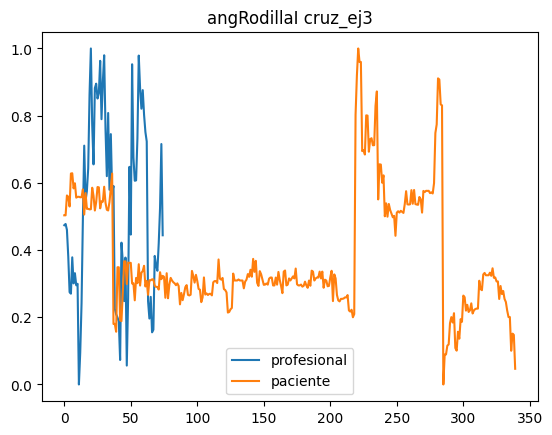
\includegraphics[width=0.8\linewidth]{img/longitud}
	\caption{Secuencias de un ángulo normalizado del paciente y del profesional.}
	\label{fig:longitud}
\end{figure}
 
Los juegos de baile suelen permitir cierto margen de error al ejecutar un movimiento en un momento distinto. Esto se podría conseguir comparando cada \textit{frame} del usuario con todos los \textit{frames} de una ventana de tiempo del vídeo modelo, pero al ser un problema de velocidad y no de haber ejecutado un movimiento de baile a un ritmo incorrecto, haría que el retraso de los movimientos se fuera acumulando, por lo que no resuelve el problema.

Esto nos llevó a replantearnos las condiciones que debía cumplir un ejercicio correcto. Para que un ejercicio fuera correcto, el paciente tendría que realizar las poses correctamente, pero no es necesario que realice el ejercicio a la misma velocidad, lo que complica bastante la obtención de esa puntuación. 

\section{Investigación sobre las series temporales}
Con los nuevos criterios obtenidos se estudió que métodos se podían usar para comparar secuencias de movimientos a distintas velocidades, esto llevó a investigar sobre las series temporales.

Se encontraron dos posibles soluciones, los modelos ocultos de Markov (HMM) y el Dynamic Time Warping (DTW) \cite{dtwandhmm}. En el caso de los HMM tienen la ventaja de que podrían permitir que, en el caso de que se encontrara una forma de obtener las poses en tiempo real, se podrían usar para dar \textit{feedback} al usuario en tiempo real, además de que con grandes sets de datos ofrecen un mejor rendimiento que DTW. El problema que conllevaría haberlas usado en lugar de DTW es precisamente la cantidad de datos, en el caso de este proyecto se contó con un set de datos muy pequeño, por lo que elegimos DTW, que se podría utilizar incluso aunque solo se tuviera un vídeo modelo y un vídeo de un paciente. 

\section{Preparación de los datos}
Una vez elegido el método que se usaría para comparar los vídeos, había que preparar los datos que se iban a usar para las pruebas. Estos datos se encontraran en dos tipos de ficheros, archivos CSV y \textit{DataFrames}. Dos motivos para ello eran la protección de datos y el gran coste de computo que es obtener las posiciones del esqueleto en un vídeo. Estos ficheros contenían tanto un número que indicaba el numero de fotograma como los datos de las posiciones.

\begin{figure}
	\centering
	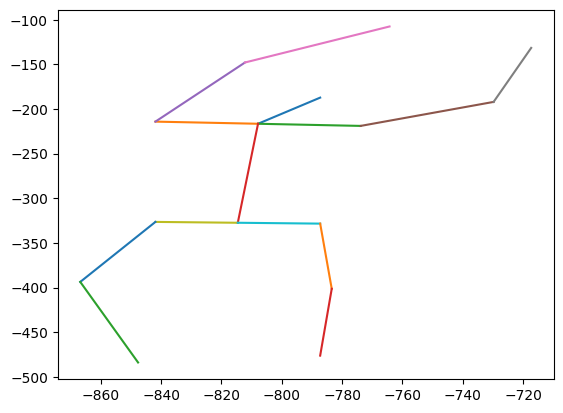
\includegraphics[width=0.7\linewidth]{img/esqueleto}
	\caption{Representación del esqueleto obtenido a partir de los puntos grabados.}
	\label{fig:esqueleto}
\end{figure}

En este caso conviene distinguir de dos tipos de datos, ángulos y coordenadas, los primeros son de una dimensión y las segundas de dos. Dependiendo del tipo de ejercicio se movían unas partes de determinada manera, este proyecto trabajo con 6 tipos de ejercicios distintos, 4 en los que se ejercitaban las piernas y 2 en los que se ejercitaban los brazos. El primer paso fue eliminar los fotogramas que tuvieran alguna posición o ángulo nulo. Para los ejemplos que se mostrarán, se han escogido vídeos de referencia de profesionales y se han comparado con los de otros profesionales y con los de los pacientes, siendo el resultado esperado el que los ejercicios de los profesionales deberían dar distancias menores y las de los pacientes distancias mayores.

No se puede utilizar DTW sin normalizarlos, ya que incluso aunque el ejercicio fuera exactamente igual, la distancia seria distinta de 0, como puede observarse en la figura \ref{fig:comparacionsinnormalizar}.  Algunas de estas posiciones contenían datos nulos, por lo que lo primero que se hizo fue descartar los nulos, ya que causaban problemas tanto en las normalizaciones que se explicaran más adelante como en el cálculo de la distancia DTW.

\begin{figure}
	\centering
	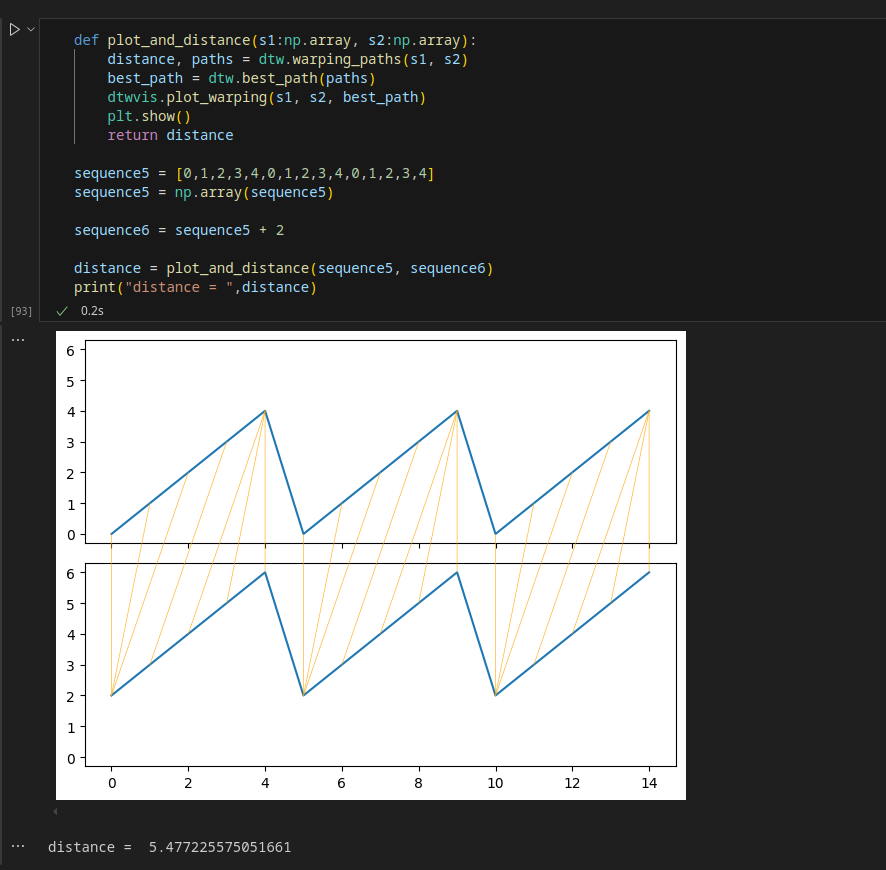
\includegraphics[width=0.7\linewidth]{img/comparacion_sin_normalizar}
	\caption{Comparación de dos secuencias sin normalizar.}
	\label{fig:comparacionsinnormalizar}
\end{figure}

\subsection{Normalización de ángulos previa}
En el caso de los ángulos inicialmente se intentó dividir cada ángulo entre 180º,  pero finalmente se utilizo la normalización \textit{min-max} para que estuvieran en un rango entre 0 y 1, ya que con los grados no se obtenían los resultados deseados.

\subsection{Normalización de coordenadas previa}
En el caso de los puntos del cuerpo era necesario normalizarlos ya que no todos los fotogramas se encontraban centrados, por lo que era necesario aplicar traslación. 

Además, había que garantizar que la traslación no generara que los números fueran negativos para que DTW diera unos resultados aceptables, por ello se aplicó traslación a cada punto  mediante el uso de una caja delimitadora por cada esqueleto de cada fotogramas de forma que todos los puntos estén en las cajas y traslada haciendo que el vértice con menores coordenadas sea el $(0,0)$.

También había otro problema, no todas las personas miden lo mismo, por lo que había que rescalar los datos. Para ello se uso la normalización L2 en cada secuencia de puntos de una parte del cuerpo, normalización explicada en \ref{norml2}. 

\section{Obtención de una distancia}
Una vez que se tenían los datos normalizados era necesario obtener la distancia DTW.  En el caso de los ángulos, al ser de una sola dimensión se aplicó DTW directamente, para ello se calculó las distancias de cada ángulo y se hizo la media de estas. En el caso de las coordenadas, que eran de dos dimensiones, se redimensionaron a vectores de una dimensión.

\begin{table}
	\centering
	\begin{tabular}{|c|c|c|c|}
		\hline
		\textbf{Tipo}  & \textbf{Distancia de posiciones} & \textbf{Distancia de ángulos}\\
		\hline
		Profesional & 0,1763 & 1,7774 \\
		\hline
	    Profesional & 0,2968 & 2,3090 \\
		\hline
		Profesional & 0,2353 & 1,6997 \\
		\hline
		Paciente & 0,5595 &  2,3495 \\
		\hline
		Paciente & 0,5366 & 2,1405 \\
		\hline
		Paciente  & 0,5356 & 2,9488 \\
		\hline
		Paciente & 0,5122 &  2,6827 \\
		\hline
	    Paciente & 0,4850 & 3,1227 \\
		\hline
		Paciente & 0,4722 & 3,3067 \\
		\hline
	\end{tabular}
	\caption{Distancias obtenidas usando todas las partes y todos los ángulos de los pacientes y profesionales.}
	\label{tab:alldistances}
\end{table}

Como inicialmente no se disponían de los datos del terapeuta, se probó a comparar las distancias obtenidas mediante la aplicación de DTW sobre ejercicios de un mismo tipo con los de distintos ejercicios. Los resultados no fueron los esperados, lo cual puede ser porque en varios de los ejercicios los movimientos son similares y como inicialmente no se filtraban que partes del cuerpo eran importantes para cada tipo de ejercicio, los resultados podían no ser fiables, por ejemplo, en dos ejercicios distintos en los que el paciente esta sentado mientras mueve una pelota con los brazo de distinta manera, comparar las piernas no aportaría información relevante. 

Una vez obtenidos los vídeos del terapeuta, se calcularon las distancias, los resultados son los de la tabla \ref{tab:alldistances}. Como se puede observar, las distancias de los ángulos son más altas que las calculadas a través de las posiciones. Se probó con otras normalizaciones como la \textit{Z-score} y dividirlo entre 180º, pero los resultados seguían sin ser aceptables por la misma razón.

Algo que hay que destacar es que en el caso de las distancias de las posiciones de los profesionales, todas ellas son inferiores a las de los pacientes, lo que tiene sentido, ya que una persona sana normalmente va a ejecutar el ejercicio mejor que una con \textit{Parkinson}.

Después, se tuvo en cuenta la posibilidad de que algunas zonas del cuerpo no se ejercitaran en algún ejercicio, por lo que se filtro que partes eran las importantes, para ello se observó cada vídeo y se guardaron los nombres de las partes ejercitadas. Un ejemplo de los resultados de seleccionar solo las partes importantes se pueden ver en la tabla \ref{tab:useddistances}.

\begin{table}
	\centering
	\begin{tabular}{|c|c|c|c|}
		\hline
		\textbf{Tipo}  & \textbf{Distancia de posiciones} & \textbf{Distancia de ángulos} \\
		\hline
		Profesional &  0,1816 & 1,2235 \\
		\hline
		Profesional &  0,3139 & 1,8826 \\
		\hline
		Profesional & 0,2665 & 1,4767 \\
		\hline
		Paciente &  0,5085 & 1,1993 \\
		\hline
		Paciente & 0,4874 & 2,1663 \\
		\hline
		Paciente  & 0,4929 & 1,3368 \\
		\hline
		Paciente & 0,4746 & 2,2297 \\
		\hline
		Paciente & 0,4425 & 1,9711 \\
		\hline
		Paciente & 0,4283 & 2,9705 \\
		\hline
	\end{tabular}
	\caption{Distancias obtenidas con solo las partes importantes para ese ejercicio de pacientes y profesionales.}
	\label{tab:useddistances}
\end{table}

\section{Puntuar un ejercicio}
Una vez obtenida la distancia, es necesario obtener la puntuación, la cuál será opuesta a la distancia, cuanto mejor sea la ejecución del ejercicio menor será la distancia y más alta la puntuación. El problema es que para ello, hay que encontrar la mayor distancia de cada caso.

En el caso de los ángulos no fue posible, ya que no se conseguía que la distancia estuviera en un rango, por lo que los resultados de ejercicios mal ejecutados eran negativos debido a que la distancia era muy alta.

En el caso de las posiciones, fue sencillo, se aplicó  a cada distancia la formula \ref{formuladist}, esto permite que la distancia 0 tenga una puntuación de 100. 
\begin{equation}
	puntuación = 100-100*distancia
	\label{formuladist}
\end{equation}

Y por último se calculaba la media de ellas. Los resultados se pueden ver en la tabla  \ref{ tab:usedscore}. Hay que tener en cuenta de que en el caso de que la media de las distancias fuera mayor que 1 la puntuación sería negativa, pero en ninguno de los ejercicios ha ocurrido, por lo que no se ha considerado un problema.
\begin{table}
	\centering
	\begin{tabular}{|c|c|}
		\hline
		\textbf{Tipo}  & \textbf{Puntuación de posiciones}\\
		\hline
		Profesional & 81,8400 \\
		\hline
		Profesional & 68,6029 \\
		\hline
		Profesional & 73,3486 \\
		\hline
		Paciente & 49,1500 \\
		\hline
		Paciente & 51,2527 \\
		\hline
		Paciente & 50,7087 \\
		\hline
		Paciente & 52,5366 \\
		\hline
		Paciente & 55,7411 \\
		\hline
		Paciente & 57,1680 \\
		\hline
	\end{tabular}
	\caption{Puntuaciones obtenidas de las posiciones de profesionales y pacientes.}
	\label{ tab:usedscore}
\end{table}

\label{obtpunt}

\section{Otras pruebas}
Durante la obtención de una distancia, se plantearon otros métodos, pero aunque los resultados que daban son muy similares, se escogió el método explicado en la sección \ref{obtpunt}.

Primero se estudió si era mejor redimensionar las series de posiciones de dos dimensiones $X$ e $Y$ a una sola o no hacerlo y aplicar DTW a cada dimensión por separado. Los resultados se pueden ver en la tabla \ref{tab:tryscore1}. Las puntuaciones son muy similares.

Otra opción era tratar el conjunto de series de posiciones de dos dimensiones redimensionadas a una dimensión como series multidimensionales. Esto se consigue mediante una implementación que ofrece la librería Dtaidistance importando el modulo \textit{ndim}. También se probo nuevamente a tratar las dimensiones $X$ e $Y$ por separado no redimensionandolas para ver si se conseguían mejores resultados. Estos resultados se pueden observar en la tabla \ref{tab:tryscore2}.

\begin{table}
	\centering
		\begin{tabular}{|c|c|c|c|c|}
			\hline
			   \textbf{Tipo}     & \textbf{Puntuación usada} & \textbf{Dimensiones divididas} \\ \hline
			 Profesional &       89,2996  & 95,9421   \\ \hline
			 Paciente &       23,3773  &  29,4185   \\ \hline
			 Paciente &       18,9154  & 25,5778   \\ \hline
			 Paciente   &       19,1309  & 25,3962   \\ \hline
			 Paciente   &       24,9134  & 31,1506   \\ \hline
			 Paciente   &       45,5613  &  45,1792   \\ \hline
			 Paciente   &       26,09757  &  35,1118   \\ \hline
			 Paciente   &       22,19180 &  31,4718   \\ \hline
			 Paciente   &       23,2319  & 31,4716   \\ \hline
			 Paciente   &		26,2338  & 36,6816 \\ \hline
			 Paciente   &		44,6043  & 49,1532 \\ \hline

		\end{tabular}
	\caption{Comparación de puntuación obtenida redminesionando cada una de las partes y de la puntuación calculando cada dimensión por separado.}
	\label{tab:tryscore1}
\end{table}

\begin{table}
	\centering
		\begin{tabular}{|c|c|c|c|c|}
			\hline
			   \textbf{Tipo}     & \textbf{Puntuación usada} & \textbf{Ndim} & \textbf{Ndim sin } \\ 
			    ~    &  ~ & \textbf{ redimenionadas} & \textbf{redimensionar} \\ \hline
			   
			 Profesional &       89,2996  & 95,3474 &  96,1810   \\ \hline
			 Paciente &       23,3773   & 66,1234 &  42,26262   \\ \hline
			 Paciente &       18,9154  & 64,2140 &  39,1279   \\ \hline
			 Paciente   &       19,1309  & 63,9295 &  38,5238   \\ \hline
			 Paciente   &       24,9134  & 68,1069 &  43,9163   \\ \hline
			 Paciente   &       45,5613   & 75,2601 &  54,6122   \\ \hline
			 Paciente   &       26,09757   & 62,0344 &  42,3221   \\ \hline
			 Paciente   &       22,19180  & 59,7707 &  38,8841   \\ \hline
			 Paciente   &       23,2319  & 59,5271 &  37,9471   \\ \hline
			 Paciente   &		26,2338  & 64,5063 &  44,8041	\\ \hline
			 Paciente   &		44,6043  & 73,8300 &  56,0422	\\ \hline

		\end{tabular}
	\caption{Puntuaciones obtenida de series multivariantes redimensionando las dimensiones X e Y y sin redimensionarlas.}
	\label{tab:tryscore2}
\end{table}



\section{Desarrollo de la aplicación}
Inicialmente se considero desarrollar una aplicación de escritorio con la que el usuario pudiera instalar la aplicación, para ello se consideraron las siguientes librerías:
\begin{enumerate}
	\item \textbf{Tkinter}: Es una librería gráfica que viene instalada por defecto en \textit{Python}, pero su  interfaz esta desactualizada, especialmente en \textit{Linux}, donde tampoco ofrece soporte para \textit{Wayland}, por lo que sería un problema de cara a futuro.
	\item \textbf{GTK}: Es una \textit{framework} gráfico muy utilizado en \textit{Linux} y es de código abierto, pero no se ha encontrado información oficial sobre como dar soporte a otros sistemas como por ejemplo \textit{Windows}.
	\item \textbf{QT}: Este \textit{framework} ofrece varias licencias para poderlo utilizar, pero puede ser complejo saber cual utilizar, otra desventaja era que no se aplican correctamente los estilos en entornos que usan \textit{GTK} como por ejemplo en \textit{Gnome}.
\end{enumerate}
Por ello se cambió de idea y se decidió desarrollar una aplicación web, lo cual permitiría que los pacientes pudieran utilizarla sin que tuvieran que instalar nada y soluciona problemas de compatibilidad entre distintos sistemas operativos. Además, gracias al uso de contenedores \textit{Docker} se puede ejecutar en un entorno local de forma sencilla.

Para ello se eligió el \textit{framework} Angular, esto ofrece la ventaja de que al ser del lado del cliente actuaría como interfaz gráfica para utilizar la API, permitiría separar la lógica del \textit{backend} del \textit{frontend}. Además, existe una librería para este \textit{framework} llamada Angular Material que permite la creación de varios componentes utilizados como por ejemplo selectores. El uso de este \textit{framework} trajo retos como fueron aprender a utilizarlo y aprender \textit{Typescript}, que es un lenguaje que no se imparte en la carrera.

Para el desarrollo de la API se optó por \textit{FastAPI}, un \textit{framework} de \textit{Python} que ofrece ventajas como el poder utilizar el patrón DTO por media de los esquemas de \textit{Pydantic}. Para la base de datos se escogió \textit{PostgreSQL} y la librería de \textit{Python SQLAlchemy}. 

La integración con \textit{Docker} trajo retos, el primero de ellos fue que al ejecutarlo por primera vez el contenedor del \textit{backend} antes de que se hubiera creado la base de datos, lo que producía un error. Finalmente se solucionó comprobando que esta se hubiera creado por medio de un comando que permite ver el estado de la base de datos. 

Otro contratiempo fue el almacenamiento de los archivos en la base de datos, en el caso de los vídeos eran demasiado grandes, por lo que  se eligió guardarlos en una carpeta con un nombre aleatorio y guardar ese nombre en la base de datos, por lo que se investigó como hacer persistente una carpeta en \textit{Docker}.

Por ultimo, los vídeos de los ejercicios estaban codificados en un \textit{codec} que no era compatible con navegadores, por lo que se utilizó \textit{ffmpeg} para codificar los vídeos a un formato compatible, concretamente el siguiente comando \ref{ffmpeg}.

\begin{figure}
\begin{lstlisting}[language=Bash]
	ffmpeg -i input_vídeo.mp4 -brand mp42 output_vídeo.mp4
\end{lstlisting}
\caption{Comando para poder ver un vídeo no compatible con navegadores en ellos}
\label{ffmpeg}
\end{figure}

El resultado de este desarrollo ha sido una aplicación web que permite a los usuarios crear una cuenta e iniciar sesión para poder ver vídeos de los ejercicios ya creados y subir sus ficheros para que se comparen con los de los profesionales y les devuelva una puntuación como se puede ver en la imagen \ref{fig:compararej}.

\begin{figure}
	\centering
	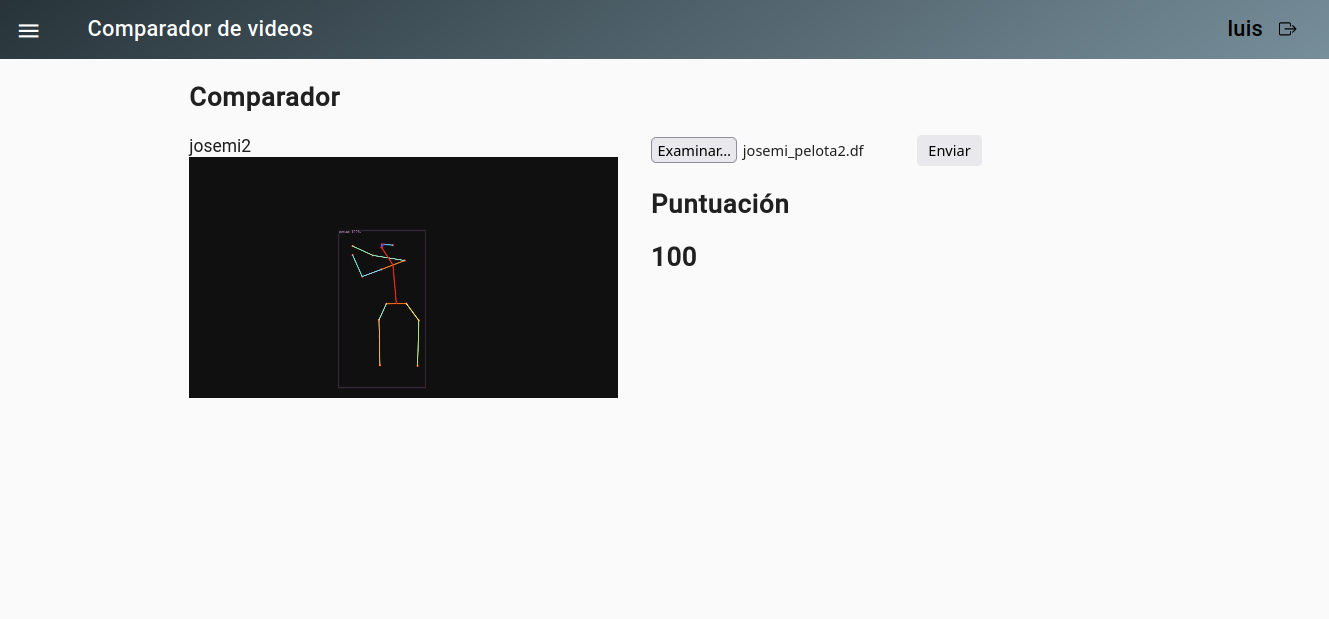
\includegraphics[width=0.7\linewidth]{img/comparar_ej}
	\caption{Comparación de ejercicio.}
	\label{fig:compararej}
\end{figure}


Para crear un ejercicio es necesario se administrador, para ello la aplicación crea una cuenta de usuario por defecto, que puede ser usada para crear ejercicios, introduciendo el nombre, añadiendo un fichero de datos, el vídeo y seleccionando ángulos y coordenadas que serán usando para comparar el ejercicio como se puede ver en la imagen \ref{fig:nuevoej}. También puede borrar ejercicios.

\begin{figure}
	\centering
	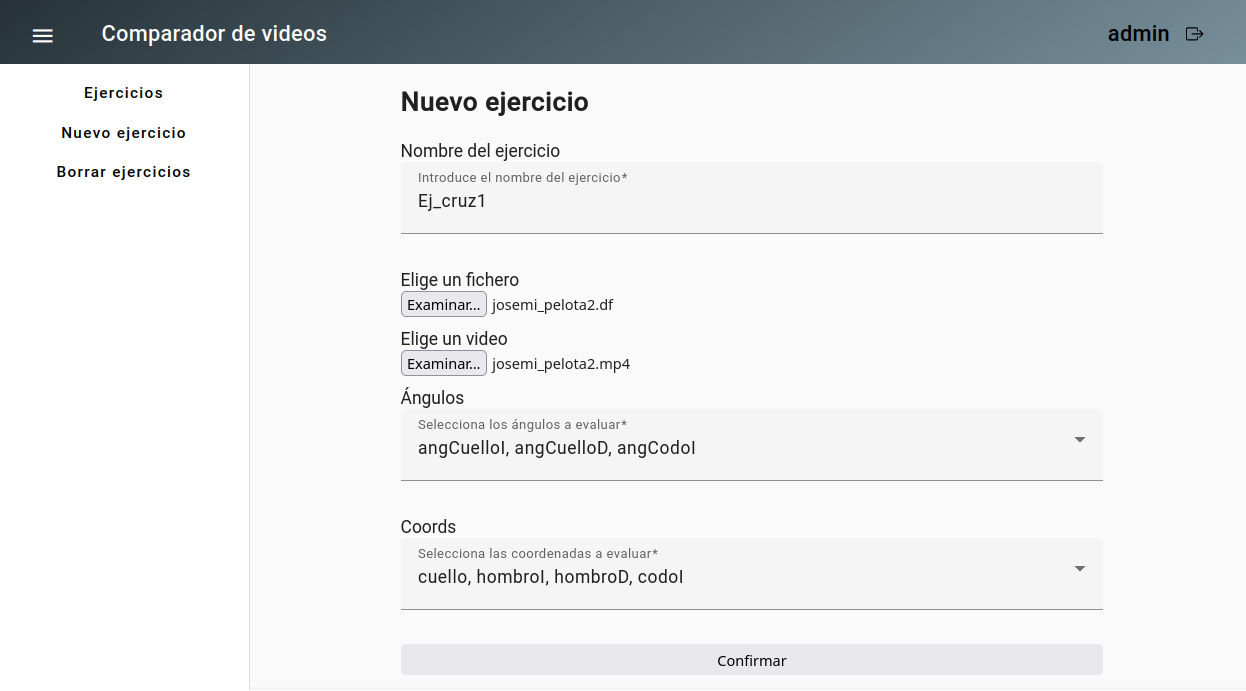
\includegraphics[width=0.7\linewidth]{img/nuevo_ej}
	\caption{Vista de nuevo ejercicio.}
	\label{fig:nuevoej}
\end{figure}